\documentclass[10pt]{beamer}

%%%
% PREAMBLE FOR THIS DOC 
%%%
%https://tex.stackexchange.com/questions/68821/is-it-possible-to-create-a-latex-preamble-header
\usepackage{/Users/miw267/Repos/csci246_fall2025/slides/preambles/beamer_preamble_for_CSCI246}



%%% TRY TO RESHOW TOC AT EACH SECTION START (with current section highlighted)
% Reference: https://tex.stackexchange.com/questions/280436/how-to-highlight-a-specific-section-in-beamer-toc
\newcommand\tocforsect[2]{%
  \begingroup
  \edef\safesection{\thesection}
  \setcounter{section}{#1}
  \tableofcontents[#2,currentsection]
  \setcounter{section}{\safesection}
  \endgroup
}


%%%% HERES HOW TO DO IT CORRECTLY
% FIRST IN .STY FILE, DO
%\usetheme[sectionpage=none]{metropolis}
% THEN AT EACH SECTION DO
%\begin{frame}{Outline}
%  \tableofcontents[currentsection]	
%\end{frame}



%\setbeamertemplate{navigation symbols}{}
%\setbeamertemplate{footline}[frame number]{}


%%%
% DOCUMENT
%%%

\begin{document}

%\maketitle

%% Title page frame
%\begin{frame}
%    \titlepage 
%\end{frame}





\title{09/15/2025: Quantifiers}
\author{CSCI 246: Discrete Structures}
\date{Textbook reference: Sec. 11, Scheinerman}

\begin{frame}
    \titlepage 
\end{frame}


\begin{frame}
%\footnotesize 
%\begin{mygreenbox}[title=Graded Quiz Pickup]
%Quizzes are in the front of the room, grouped into four bins (A-G, H-L, M-R, S-Z) by last name. The quizzes are upside down with your last name on the back. Come find yours before, during, or after class.  Only turn the quiz over if it's yours.
%\end{mygreenbox} 
%\vfill 

\begin{myredbox}[title=Announcements]
\begin{itemize}
	\item Reminder: If you finish the quiz early, please be \underline{silent} until everyone else is finished (so as to not distract students who are still thinking).
	\item Reminder: Mike's office hours are canceled until he returns from out of town Friday 9/25.  Madhav's office hours and SmartyCats tutoring are running as normal. Feel free to contact Mike by email if you'd like.  
\end{itemize}

\end{myredbox}
\vfill 




\begin{myyellowbox}[title=Today's Agenda]
\begin{itemize}
	\item Weekly Quiz ($\approx$ 15 mins)
	\item Review group exercises ($\approx$ 10 mins)
	\item Mini-lecture ($\approx$ 15 mins)
	\item Group exercises ($\approx$ 10 mins)
\end{itemize}

\end{myyellowbox}
\vfill 

\end{frame}


\begin{frame}
%\small 
 \begin{myredbox}[title=Weekly Quiz \#3] 
\begin{enumerate}
	\item  \textit{(Sec. 7 -- Boolean Algebra.)} DeMorgan's laws are:
	\[ \lnot (x \land y) = (\lnot x) \lor (\lnot y) \quad \text{and} \quad \lnot (x \lor y) = (\lnot x) \land (\lnot y). \]
	Prove the first of these (using truth tables). For reference: $\lnot$ means \qq{not}, $\land$ means \qq{and}, and $\lor$ means \qq{or}.
	\item  \textit{(Sec. 8 -- Lists.)}  We have a club with 20 members. We want to elect an executive board consisting of a president, a vice president, a secretary, and a treasurer.  How many ways can we do this (assuming no member of the club can fill two offices)?
    \item \textit{(Sec. 9 -- Factorial.)}
%    \vspace{-.5cm}
%    \begin{columns}[t] % top-aligned columns
%        \begin{column}{0.7\textwidth}
%            \qquad \quad 
Your friend Sandy has 6 different books of classical literature,  7 different \textit{romantasy} (i.e. romance fantasy) books, and 8 different self-help books. (a) In how many different ways can Sandy's books be arranged on a bookshelf? (b) In how many different ways can Sandy's books be arranged on the bookshelf if all books of the same category are grouped together? 
%        \end{column}
%        \begin{column}{0.3\textwidth}
%            \vspace{0pt} % aligns top with text
%            
\includegraphics[width=\linewidth]{images/romantasy}
%        \end{column}
%    \end{columns}
\end{enumerate}
\end{myredbox}


\end{frame}



\begin{frame}{Subtopics from today's reading}
Scheinerman Sec. 11 (Quantifiers) covers the following subtopics
\begin{enumerate}
	\item Using quantified statements
	\begin{enumerate}
	\item[a.] How to interpret quantified statements
 	\item[b.] How to negate quantified statements
 	\end{enumerate}
	\item Proving quantified statements
	\begin{enumerate}
	\item[a.] Proving existential statements
	\item[b.] Proving universal statements
 	\end{enumerate}
\end{enumerate}

%In today's class, we'll focus on \#1, because it's newer.  Please make sure you can also do \#2 (see text).
\end{frame}


%%%% Section
\begin{frame}[standout]
Outline for Mini-Lecture:
\begin{itemize}
\item \alert{\textbullet \quad Using quantified statements}
\item \textbullet \quad Proving quantified statements
\item \textbullet \quad Applications
\end{itemize}
\end{frame}




\begin{frame}{}

\begin{center}
\colorbox{green!30}{\textbf{Proposition.}} $\forall \; \texttt{jar} \in \texttt{jars}, \; \exists \; \texttt{ball} \in \texttt{jar} : \texttt{ball}  \; \text{is red}$

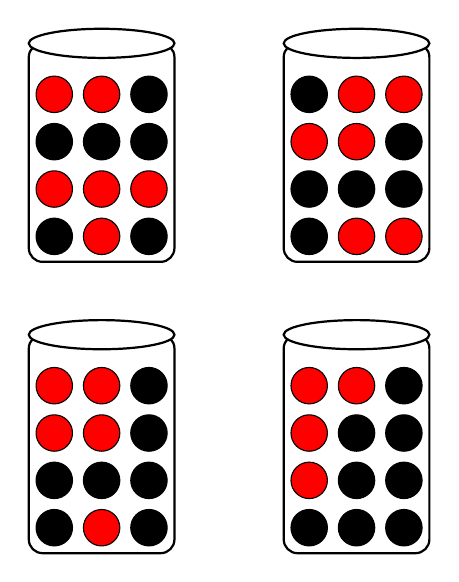
\begin{tikzpicture}[scale=0.925]
% Parameters
\def\jarwidth{2}
\def\jarheight{3}
\def\ballradius{0.25}

% Jar positions for a 2x2 grid
\foreach \i in {0,1} {
    \foreach \j in {0,1} {
        \begin{scope}[shift={(\i*3.5,-\j*4)}]
            % Draw jar rectangle
            \draw[thick, rounded corners=5pt] (0,0) rectangle (\jarwidth,\jarheight);

            % Draw jar opening (ellipse at top)
            \draw[thick, fill=white] (\jarwidth/2, \jarheight) ellipse (\jarwidth/2 and 0.2);

            % Place balls in a 3x3-ish grid inside the jar
            \foreach \x in {0.35,1.0,1.65} {
                \foreach \y in {0.35,1.0,1.65,2.3} {
                    % Decide color: mostly black, some red
                    \pgfmathsetmacro\colorprob{rand}
                    \ifdim \colorprob pt<0.15pt
                        \edef\ballcolor{red} % 1 or 2 red balls
                    \else
                        \edef\ballcolor{black}
                        
                    \fi
                    \fill[\ballcolor] (\x,\y) circle (\ballradius);
                    \draw (\x,\y) circle (\ballradius);
                }
            }
        \end{scope}
    }
}
\end{tikzpicture}
\end{center}

\only<1-2>{\colorbox{yellow!30}{\textbf{Poll.}} What is the proposition saying in English? \\}  
\vfill 

\only<2>{\colorbox{green!30}{\textbf{Solution.}}  For each jar in the set of jars, there is a ball in the jar such that the ball is red.} 

\only<3-4>{\colorbox{yellow!30}{\textbf{Poll.}} Is this proposition true or false? \\}  
\vfill 

\only<4>{\colorbox{green!30}{\textbf{Solution.}}  True} 

\only<5-6>{\colorbox{yellow!30}{\textbf{Poll.}} How can we change the picture to make the proposition false? \\}   
\vfill 
\only<6>{\colorbox{green!30}{\textbf{Solution.}}  We need to change one of the jars so that it has no red balls.}
\end{frame}



\begin{frame}{}

\begin{center}
\colorbox{green!30}{\textbf{Proposition.}} $\forall \; \texttt{jar} \in \texttt{jars}, \; \exists \; \texttt{ball} \in \texttt{jar} : \texttt{ball}  \; \text{is red}$

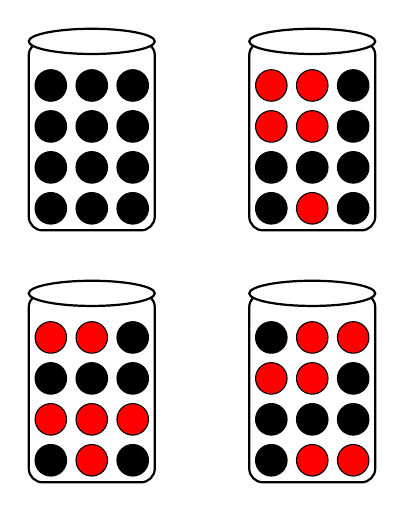
\begin{tikzpicture}[scale=0.8]
% Parameters
\def\jarwidth{2}
\def\jarheight{3}
\def\ballradius{0.25}

% Jar positions for a 2x2 grid
\foreach \i in {0,1} {
    \foreach \j in {0,1} {
        \begin{scope}[shift={(\i*3.5,-\j*4)}]
            % Draw jar rectangle
            \draw[thick, rounded corners=5pt] (0,0) rectangle (\jarwidth,\jarheight);

            % Draw jar opening (ellipse at top)
            \draw[thick, fill=white] (\jarwidth/2, \jarheight) ellipse (\jarwidth/2 and 0.2);

            % Place balls in a 3x3-ish grid inside the jar
            \foreach \x in {0.35,1.0,1.65} {
                \foreach \y in {0.35,1.0,1.65,2.3} {
                    % Determine color
                    \ifnum\i=0\relax
                        \ifnum\j=0\relax
                            % Top-left jar: all black
                            \def\ballcolor{black}
                        \else
                            % Other jars: mostly black with a few red
                            \pgfmathsetmacro\colorprob{rand}
                            \ifdim \colorprob pt<0.15pt
                                \def\ballcolor{red}
                            \else
                                \def\ballcolor{black}
                            \fi
                        \fi
                    \else
                        % Other jars
                        \pgfmathsetmacro\colorprob{rand}
                        \ifdim \colorprob pt<0.15pt
                            \def\ballcolor{red}
                        \else
                            \def\ballcolor{black}
                        \fi
                    \fi

                    % Draw the ball
                    \fill[\ballcolor] (\x,\y) circle (\ballradius);
                    \draw (\x,\y) circle (\ballradius);
                }
            }
        \end{scope}
    }
}
\end{tikzpicture}

\end{center}

\only<1-2>{\colorbox{yellow!30}{\textbf{Poll.}} What is the proposition saying in English? \\}  
\vfill 

\only<2>{\colorbox{green!30}{\textbf{Solution.}}  For each jar in the set of jars, there is a ball in the jar such that the ball is red.} 

\only<3-4>{\colorbox{yellow!30}{\textbf{Poll.}} Is this proposition true or false? \\}  
\vfill 

\only<4>{\colorbox{green!30}{\textbf{Solution.}}  False.} 

\only<5-7>{\colorbox{yellow!30}{\textbf{Poll.}} How can we change the proposition to make it true? \\}   
\vfill 
\only<6-7>{\colorbox{green!30}{\textbf{Solution.}} 
$\lnot \bigg( \forall \; \texttt{jar} \in \texttt{jars}, \; \exists \; \texttt{ball} \in \texttt{jar} : \texttt{ball}  \; \text{is red} \bigg)$ \\}
\only<7>{That is, $\bigg( \exists \; \texttt{jar} \in \texttt{jars}, \; : \; \forall \; \texttt{ball} \in \texttt{jar} : \texttt{ball}  \; \text{is NOT red} \bigg).$ 	
}
\end{frame}

\begin{frame}{Negating quantified statements}
\footnotesize 

\colorbox{green!30}{\textbf{Big Picture.}}To negative quantified statements, \qq{flip} the quantifiers and carry the \qq{not} operator through.

 
\vfill 

\begin{mygreenbox}[title=Negating \textbf{Existential} Statements]
\begin{align*}
\lnot \bigg( \exists x \in A, \text{assertions about x}\bigg) &&\text{is the same as} \\
\forall x \in A, \lnot \bigg( \text{assertions about x}\bigg)	
\end{align*}	
\end{mygreenbox}
\pause 
\vfill 
\begin{mygreenbox}[title=Negating \textbf{Universal} Statements]
\begin{align*}
\lnot \bigg( \forall x \in A, \text{assertions about x}\bigg) &&\text{is the same as} \\
\exists x \in A, \lnot \bigg( \text{assertions about x}\bigg)	
\end{align*}	
\end{mygreenbox}
\pause 
\vfill 
\colorbox{red!30}{\textbf{Remark.}} This technique applies even if there are multiple quantifiers (as we saw in the jars slide).  \pause E.g. $\lnot \bigg( \exists \cdots : \forall \cdots,  \exists \cdots : \forall \cdots, \texttt{something} \bigg)$ is the same as  $\bigg( \forall \cdots , \exists \cdots  : \forall \cdots , \exists \cdots : \texttt{NOT something} \bigg)$.
\end{frame}



%%%% Section
\begin{frame}[standout]
Outline for Mini-Lecture:
\begin{itemize}
\item \textbullet \quad Using quantified statements
\item \alert{\textbullet \quad Proving quantified statements}
\item \textbullet \quad Applications
\end{itemize}
\end{frame}


\begin{frame}{Proving existential statements}

\colorbox{red!30}{\textbf{Proposition.}} There is an integer that is even and prime.

\vfill 
\pause 
\colorbox{yellow!30}{\textbf{Poll.}} How to express the proposition in quantified form?

\vfill 
\pause 

\colorbox{green!30}{\textbf{Proposition (with quantifiers).}} $\exists \; x \in \mathbb{Z} : x \text{ is even and prime}$. 

\vfill 
\pause 


\colorbox{yellow!30}{\textbf{Poll.}} How to prove the proposition?

\vfill 
\pause 

\colorbox{green!30}{\textbf{Solution.}} Consider the integer 2.  The integer 2 is both even and prime.  (Here you could possibly justify these properties via the definitions.)

\vfill 
\pause 
\colorbox{red!30}{\textbf{Remark.}} Proving an existential statement is \alert{akin to finding a counterexample.} 

\vfill 
\pause 

\colorbox{blue!30}{\textbf{General strategy.}}
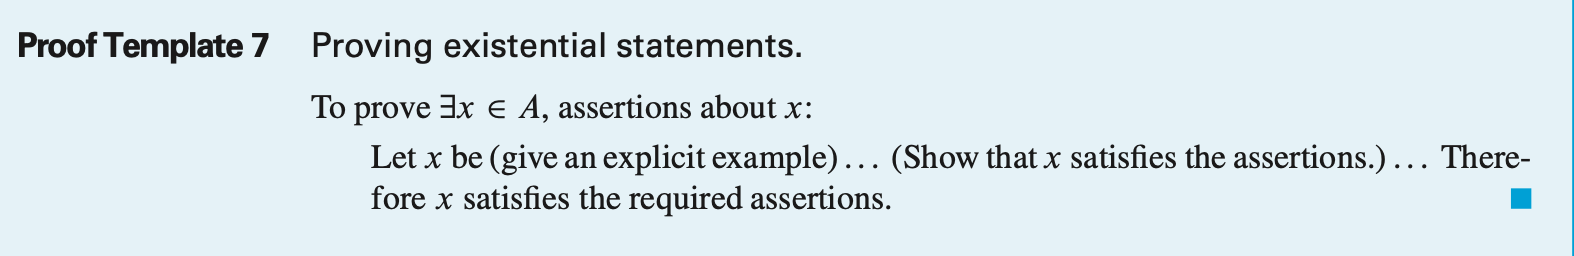
\includegraphics[width=\textwidth]{images/proving_existential.png}


	
\end{frame}



\begin{frame}{Proving universal statements}

\colorbox{red!30}{\textbf{Proposition.}} Every integer that is divisible by 6 is even.

\vfill 
\pause 
\colorbox{yellow!30}{\textbf{Poll.}} How to express the proposition in quantified form?

\vfill 
\pause 

\colorbox{green!30}{\textbf{Proposition (with quantifiers).}} Let $A = \set{x \in \mathbb{Z} : 6 \mid x}$.  Then  $\forall \; x \in A,$ $x$ is even.

\vfill 
\pause 


\colorbox{yellow!30}{\textbf{Poll.}} How to prove the proposition?

\vfill 
\pause 

\colorbox{green!30}{\textbf{Solution.}} Let $x \in A$. Then there is an integer $y$ such that $x=6y$. \pause We can rewrite this as $x=2(3y)$. \pause  Since $3y$ is an integer, x is divisible by 2, and therefore even.

\vfill 
\pause 
\colorbox{red!30}{\textbf{Remark.}} Proving an universal statement is \alert{akin to proving an if-then statement.} (\qq{If $x$ is divisible by 6, then $x$ is even}.)

\vfill 
\pause 

\colorbox{blue!30}{\textbf{General strategy.}}
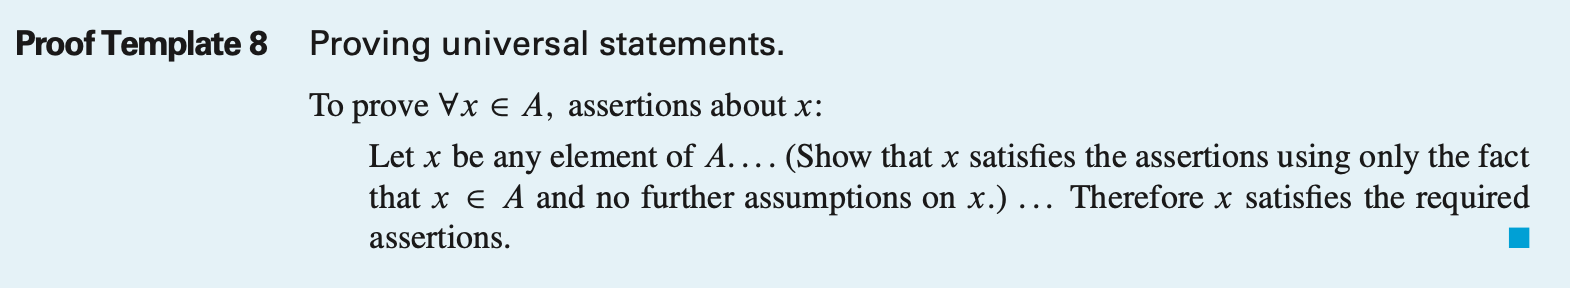
\includegraphics[width=\textwidth]{images/proving_universal.png}


	
\end{frame}


\begin{frame}

 \begin{myyellowbox}[title=Puzzle]
Evaluate the (partial) student solution below. 
\end{myyellowbox}

\vfill 

 \begin{mygreenbox}[title=Quiz Question (Quantifiers) from Spring 2025]
Let $A = \set{x \in \mathbb{Z}: 6|x}$.  Prove that $\forall x \in A, $ x is even.
\end{mygreenbox}
\vfill 

\vfill 
 \begin{myredbox}[title=(Partial) Student Solution]

\begin{align}
A = \set{x \in \mathbb{Z}: 6|x} \\
\exists y : \forall x, \; x=6y
\end{align}
\end{myredbox}
\pause 
\vfill 
 \begin{myyellowbox}[title=Comments]
Line 2 in the solution is \texttt{False}. 

\[ \explaintermbrace{there exists}{\exists} y  \;\explaintermbrace{such that}{:} \; \explaintermbrace{for all}{\forall} x, \; x=6y \] 
 (No matter what you pick for $y$, $6y$ can't represent all integers).
\end{myyellowbox}

\end{frame}


\begin{frame}{Solution Sketch}
\footnotesize 
 \begin{myyellowbox}[title=General Observation]
The primary issue (even to students who scored 4/4) was \textbf{communication} -- that is structuring the mathematical argument clearly. 
%Note that you can just reuse the old if-then proof template.
\end{myyellowbox}
\vfill 
 \begin{mygreenbox}[title=\text{Solution Using The If-Then Proof Template.}]
\textbf{Proposition.} Let $A = \set{x \in \mathbb{Z}: 6|x}$.  Then $\forall x \in A, $ x is even.

\vspace{0.25cm}

\textbf{Proof.}

\begin{tabularx}{\textwidth}{|L{3cm}|X|}
\hline \textbf{Annotation} & \textbf{Main Text} \\ \hline
 \hlorange{Convert Prop. to ``if-then" form} &  \hlorange{We show that if $x \in A$, then $x$ is even.} \\ \hline
\hlblue{State assumption} & \hlblue{Suppose $x \in A$.} \\ \hline
\hlgreen{Unravel defs.} & \hlgreen{So $6|x$.  That is, there is an integer $c$ such that $x=6c$.} \\ \hline
\hlred{*** The glue ***} & \hlred{We can write $x=6c=2(3c)$.} \\ \hline
 \hlgreen{Unravel defs.} & \hlgreen{So there is an integer $d \red{(=3c)}$ such that $x=2d$. In other words, $2|x$.  } \\ \hline
  \hlblue{State conclusion.} & \hlblue{So, $x$ is even.} \\ \hline
\hline
\end{tabularx}
\end{mygreenbox}
\end{frame}

%%%% Section
\begin{frame}[standout]
Outline for Mini-Lecture:
\begin{itemize}
\item \textbullet \quad Using quantified statements
\item \textbullet \quad Proving quantified statements
\item \alert{\textbullet \quad Applications}
\end{itemize}
\end{frame}

\begin{frame}{Application Ex. 1: Graph Theory}
\small 

\begin{center}
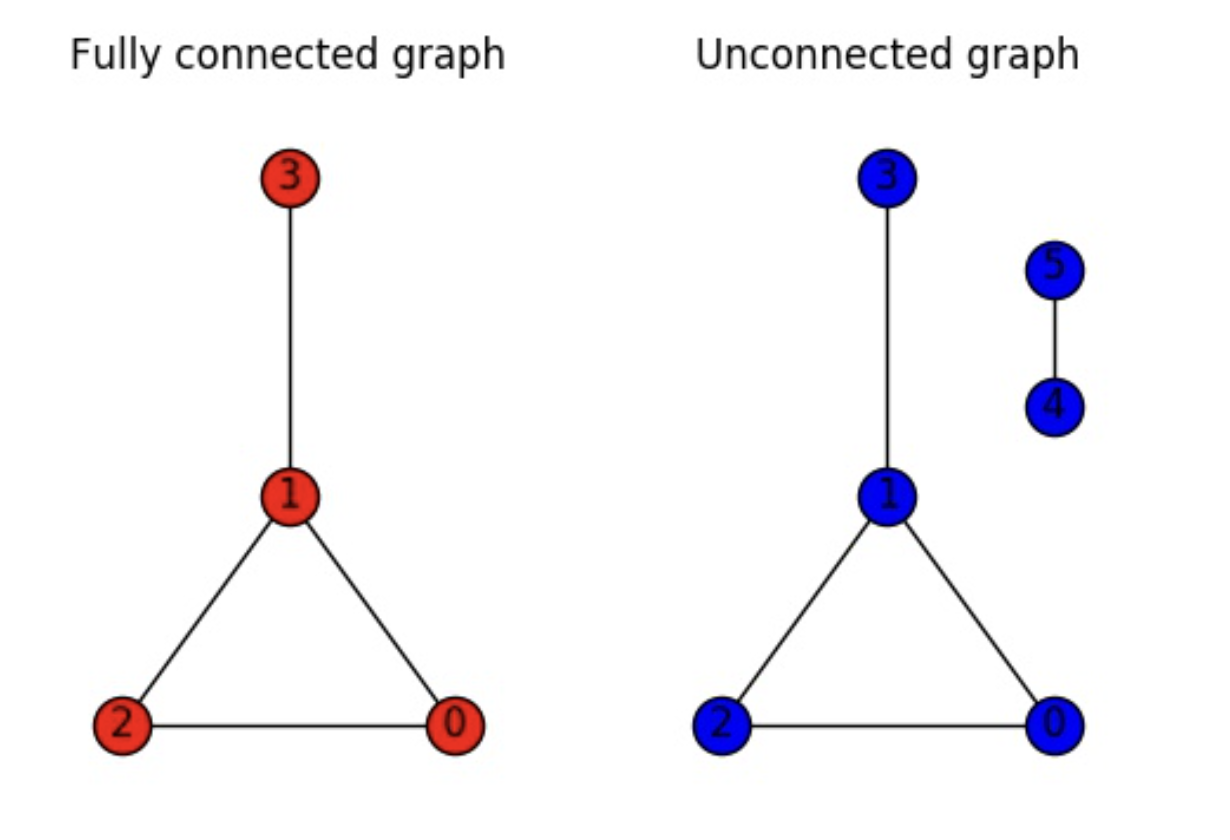
\includegraphics[width=.6\textwidth]{images/connected_graph.png}	
\end{center}
\pause 

\vfill 
\vspace{-.5cm}

\begin{mygreenbox}[title=Definition]
A graph $G$ is connected if %every pair of vertices is reachable.

\[\forall u,v \in \texttt{Vertices}(G), \;  \exists \, \text{ path } P \text{ from } u \text{ to } v. \]
\end{mygreenbox}


\vfill 
\pause 
\colorbox{green!30}{\textbf{Translation.}} For all pairs of vertices, there exists a path connecting them. 
\vfill 
\pause 
\colorbox{red!30}{\textbf{Remark.}}   This combines universal and existential quantifiers naturally.

\end{frame}

\begin{frame}{Application Ex. 2: Randomized Algorithms}

Imagine you have a randomized algorithm $A$ that tries to solve a problem $P$, like generating a valid puzzle or finding a satisfiable solution.  \pause 
 
You might want to express that with high probability it works for all valid inputs: \pause 
%
\begin{align*}
\forall \; x \in \texttt{ValidInputs}, \forall \; \epsilon > 0, \exists N \in \mathbb{N} :  \\ Pr[\text{Algorithm $A$ solves $x$ in $N$ steps}] \geq 1 - \epsilon 	
\end{align*}



\vfill 
\colorbox{green!30}{\textbf{Translation into words.}} 
\qq{For all valid inputs $x$ and for any tiny failure probability $\epsilon$,  there exists a number of steps $N$ such that the randomized algorithm succeeds with probability at least $1-\epsilon$.}


\vfill 
\pause 
\begin{tabular}{{p{0.80\linewidth}p{0.20\linewidth}}}
  \begin{minipage}[b]{\textwidth}
 \colorbox{blue!30}{\textbf{Application.}} Finding influential samples in large datasets.   \\\scripttext{(\textbf{Woj.} et al., 2017, \textit{IEEE Big Data})}\\
  \end{minipage} &
      \centering 
\includegraphics[width=.20\textwidth]{images/needle_in_haystack.jpeg} 
\end{tabular}

\end{frame}





\begin{frame}{Random group assignments}
%%% TABLE 1: by last name
\begin{columns}
\begin{column}{0.33\textwidth}
Ashley, Isabelle: 2 \\ 
Bailey, Tanna: 3 \\ 
Blaisdell, Olyver: 4 \\ 
Brown, Ashton: 13 \\ 
Brown, Jonathan: 3 \\ 
Cardenas, Dominic: 12 \\ 
Cutler, George: 8 \\ 
Fabik, Roland: 9 \\ 
Fellows, Audrey: 5 \\ 
Fitzgerald, Ryan: 4 \\ 
Fuller, Ryan: 7 \\ 
Griffen, Clara: 7 \\ 
Grutsch, Tanner: 13 \\\end{column}
\begin{column}{0.33\textwidth}
Hager, Nathan: 11 \\ 
Horner, Jayden: 1 \\ 
Johnson, Jaret: 2 \\ 
Kintzel, Samantha: 1 \\ 
Lameres, Alexis: 8 \\ 
Lee, Holden: 6 \\ 
Mayala, Reece: 5 \\ 
McLean, Connor: 6 \\ 
Mcbride, Daniel: 11 \\ 
Miller, Maverick: 10 \\ 
Moss, Emily: 4 \\ 
Mousseau, Matthew: 10 \\ 
Neuman, Evan: 12 \\\end{column}
\begin{column}{0.33\textwidth}
Putnam, John: 6 \\ 
Ramos, Vydel: 1 \\ 
Rathbun, Jedidiah: 2 \\ 
Roberts, Matthew: 3 \\ 
Roller, Nathan: 9 \\ 
Ryan, Otis: 7 \\ 
Shevtsov, Timothy: 11 \\ 
Sinclair, Aidan: 12 \\ 
Smith, Charles: 9 \\ 
Stensland, Emma: 13 \\ 
Thiessen, Logan: 5 \\ 
Thompson, Jaiden: 10 \\ 
Vath, Ethan: 8 \\\end{column}
\end{columns}
\end{frame}


\begin{frame}{Group Exercises: Quantifiers}

\footnotesize 
\begin{minipage}{0.56\textwidth}
    1. Label each sentence below about the integers as true or false. 
    \begin{itemize}
        \item[a.] $\forall x, \forall y, x+y=0.$ 
        \item[b.] $\forall x, \exists y: x+y=0.$
        \item[c.] $\exists x: \forall y, x+y=0.$
        \item[d.] $\exists x, \exists y: x+y=0.$
        \item[e.] $\forall x, \forall y, xy=0.$
        \item[f.] $\forall x, \exists y: xy=0.$
        \item[g.] $\exists x: \forall y, xy=0.$
        \item[h.] $\exists x, \exists y: xy=0.$
    \end{itemize}
    2. The notation $\exists!$ can be read "there is a unique." Label each sentence below true or false.
    \vspace{-0.5cm}
    \begin{itemize}
        \item[a.] $\exists! x \in \mathbb{N}: x^2=4.$ 
        \item[b.] $\exists! x \in \mathbb{Z}: x^2=4.$ 
        \item[c.] $\exists! x \in \mathbb{N}: x^2=3.$ 
        \item[d.] $\exists! x \in \mathbb{Z}: \forall y \in \mathbb{Z}, xy=x.$ 
        \item[e.] $\exists! x \in \mathbb{Z}: \forall y \in \mathbb{Z}, xy=y.$ 
    \end{itemize}
\end{minipage}
\hfill
\begin{minipage}{0.38\textwidth}
    3. For each sentence below, write the negation of the sentence, but place the $\lnot$ symbol as far to the right as possible. Then rewrite the negation in English.  The first problem is done for you.
    \begin{itemize}
    
        \item[a.] $\forall x \in \mathbb{Z}, x \text{ is odd.} $  \alert{Solution: $\exists x \in \mathbb{Z}: \lnot (x \text{ is odd}.)$. In English: "There is an integer which is not odd."}
        \item[b.] $\forall x \in \mathbb{Z}, x<0.$ 
        \item[c.] $\exists x \in \mathbb{Z}: x=x+1.$
        \item[d.] $\exists x \in \mathbb{N}: x>10.$
        \item[e.] $\forall x \in \mathbb{N}, x+x=2x.$
        \item[f.] $\exists x \in \mathbb{Z}: \forall y \in \mathbb{Z}, x>y.$
        \item[g.]  $\forall x \in \mathbb{Z}, \forall y \in \mathbb{Z}, x=y.$
        \item[h.] $\forall x \in \mathbb{Z}, \exists y \in \mathbb{Z}: x+y=0.$
    \end{itemize}
\end{minipage}

\end{frame}

\begin{frame}{Solutions to Group Exercises \#1}

 Label each sentence below about the integers as true or false. 
    \begin{itemize}
        \item[a.] $\forall x, \forall y, x+y=0.$   \red{False.}  (Counter-example: $x=1, y=1$.)
        \item[b.] $\forall x, \exists y: x+y=0.$  \forestgreen{True.}  (Set $y=-x$.) 
        \item[c.] $\exists x: \forall y, x+y=0.$   \red{False.}  (Counter-example: If $x=0$, set $y=1$. If $x \neq 0$, set $y=0$.)
        \item[d.] $\exists x, \exists y: x+y=0.$  \forestgreen{True.}  (Set $x=1,y=-1$.)
        \item[e.] $\forall x, \forall y, xy=0.$  \red{False.}   (Counterexample: set $x=y=1$.)
        \item[f.] $\forall x, \exists y: xy=0.$  \forestgreen{True.}  (Set $y=0$.)
        \item[g.] $\exists x: \forall y, xy=0.$  \forestgreen{True.}  (Set $x=0$.)
        \item[h.] $\exists x, \exists y: xy=0.$  \forestgreen{True.}  (Set $x=y=0$.)
    \end{itemize}


\end{frame}


\begin{frame}{Solutions to Group Exercises \#2}

The notation $\exists!$ can be read "there is a unique." Label each sentence below true or false.

    \begin{itemize}
        \item[a.] $\exists! x \in \mathbb{N}: x^2=4.$   \forestgreen{True.}  ($x=2$ is the only solution to the equation in the natural numbers.)
        \item[b.] $\exists! x \in \mathbb{Z}: x^2=4.$   \red{False.}   ($x=2$ and $x=-2$ are two different integers which solve the equation.)
        \item[c.] $\exists! x \in \mathbb{N}: x^2=3.$   \red{False.}   (There is no solution to the equation in the set of natural numbers.)
        \item[d.] $\exists! x \in \mathbb{Z}: \forall y \in \mathbb{Z}, xy=x.$   \forestgreen{True.}  ($x=0$ is the only solution to the equation in the integers.)
        \item[e.] $\exists! x \in \mathbb{Z}: \forall y \in \mathbb{Z}, xy=y.$  \forestgreen{True.}  ($x=1$ is the only solution to the equation in the integers.)
    \end{itemize}


\end{frame}



\begin{frame}{Solutions to Group Exercises \#3 a-d}
\small 
For each sentence below, write the negation of the sentence, but place the $\lnot$ symbol as far to the right as possible. Then rewrite the negation in English.  
    \begin{itemize}    
        \item[a.] $\forall x \in \mathbb{Z}, x \text{ is odd.} $   \alert{Solution: $\exists x \in \mathbb{Z}: \lnot (x \text{ is odd})$.  In English: "There is an integer which is not odd." Alternatively, we could write the negated proposition as $\exists x \in \mathbb{Z}: (x \text{ is even})$.  In English: "There is an integer which is even."  Note: the negated proposition is}\,\forestgreen{True.} 
        \item[b.] $\forall x \in \mathbb{Z}, x<0.$  \alert{Solution: $\exists x \in \mathbb{Z}: \lnot (x<0.)$.   In English: "There is an integer which is not less than zero."  Alternatively, we could write $\exists x \in \mathbb{Z}: x \geq 0$. In English: "There is an integer which is greater than or equal to zero."   Note: the negated proposition is}\,\forestgreen{True.} 
        \item[c.] $\exists x \in \mathbb{Z}: x=x+1.$  \alert{Solution: $\forall x \in \mathbb{Z}: \lnot (x=x+1)$. That is, $\forall x \in \mathbb{Z}: (x \neq x+1)$. In English: "No integer equals one plus itself." Note: the negated proposition is}\,\forestgreen{True.} 
        \item[d.] $\exists x \in \mathbb{N}: x>10.$  \alert{Solution: $\forall x \in \mathbb{N}: \lnot (x>10)$. Alternatively, $\forall x \in \mathbb{N}: x \leq 10.$ In English: "Each natural number is less than or equal to 10."  Note: the negated proposition is}\, \red{False.} 
        \end{itemize}
\end{frame}


\begin{frame}{Solutions to Group Exercises \#3 e-h}
\small 
For each sentence below, write the negation of the sentence, but place the $\lnot$ symbol as far to the right as possible. Then rewrite the negation in English. 
    \begin{itemize}
     \item[e.] $\forall x \in \mathbb{N}, x+x=2x.$  \alert{Solution: $\exists x \in \mathbb{N}: \lnot (x+x=2x)$.  That is, $\exists x \in \mathbb{N}: x+x \neq 2x)$.  In English: "There is a natural number such that the sum of the number with itself does not equal double itself."  Note: the negated proposition is}\, \red{False.} 
        \item[f.] $\exists x \in \mathbb{Z}: \forall y \in \mathbb{Z}, x>y.$  \alert{Solution: $\forall x \in \mathbb{Z}, \exists y \in \mathbb{Z} : \lnot (x>y)$.   That is, $\forall x \in \mathbb{Z}, \exists y \in \mathbb{Z} : x\leq y$ In English: "For all integers, there is another integer which is at least as large as it."  Note: the negated proposition is}\, \forestgreen{True}.  
        \item[g.]  $\forall x \in \mathbb{Z}, \forall y \in \mathbb{Z}, x=y.$  \alert{Solution: $\exists x \in \mathbb{Z}, \exists y \in \mathbb{Z} : \lnot (x=y)$.   That is, $\exists x \in \mathbb{Z}, \exists y \in \mathbb{Z} : x\neq y$. In English: "There are two integers which do not equal each other."  Note: the negated proposition is}\, \forestgreen{True}.  
        \item[h.] $\forall x \in \mathbb{Z}, \exists y \in \mathbb{Z}: x+y=0.$  \alert{Solution: $\exists x \in \mathbb{Z}: \forall y \in \mathbb{Z} : \lnot (x+y=0)$.   That is, $\exists x \in \mathbb{Z}: \forall y \in \mathbb{Z} : (x+y \neq 0)$.  In English: "There is an integer such that the sum with all other integers does not equal zero."  Note: the negated proposition is}\, \red{False}.  

        \end{itemize}
\end{frame}


\end{document}
